\documentclass{article}
\usepackage{tikz}
\usetikzlibrary{arrows.meta,positioning,calc,shapes.geometric}
\pagestyle{empty}
\begin{document}
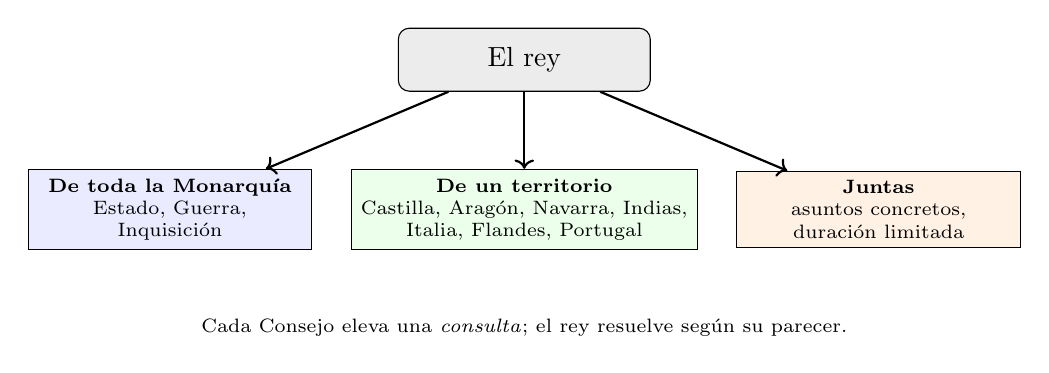
\begin{tikzpicture}
\tikzset{every node/.append style={align=center}}

\node[draw, rounded corners, fill=gray!15, minimum width=3.2cm, minimum height=0.8cm] (rey) at (6,4.2) {El rey};
\node[draw, fill=blue!8, minimum width=3.6cm, minimum height=0.9cm, align=center, font=\scriptsize] (g) at (1.5,2.3) {\textbf{De toda la Monarquía}\\Estado, Guerra,\\Inquisición};
\node[draw, fill=green!8, minimum width=4.4cm, minimum height=0.9cm, align=center, font=\scriptsize] (t) at (6,2.3) {\textbf{De un territorio}\\Castilla, Aragón, Navarra, Indias,\\Italia, Flandes, Portugal};
\node[draw, fill=orange!10, minimum width=3.6cm, minimum height=0.9cm, align=center, font=\scriptsize] (j) at (10.5,2.3) {\textbf{Juntas}\\asuntos concretos,\\duración limitada};
\draw[->, thick] (rey) -- (g); \draw[->, thick] (rey) -- (t); \draw[->, thick] (rey) -- (j);
\node[font=\scriptsize, align=center] at (6,0.8) {Cada Consejo eleva una \emph{consulta}; el rey resuelve según su parecer.};

\end{tikzpicture}
\end{document}
